\documentclass{beamer}
\usepackage[french]{babel}
\usepackage{beamerthemesplit} % new 
\usepackage[utf8]{inputenc}
\usepackage{tabularx} % in the preamble
\usepackage{listings}
\usetheme{Warsaw}
\begin{document}
\lstset{
	tabsize=4,
	language=Java,
        basicstyle=\scriptsize,
        columns=fixed,
        extendedchars=true,
        breaklines=true,
		frame=single,
        showtabs=false,
        showspaces=false,
        showstringspaces=false,
        identifierstyle=\ttfamily,
        keywordstyle=\color[rgb]{0,0,1},
        commentstyle=\color[rgb]{0.133,0.545,0.133},
        stringstyle=\color[rgb]{0.627,0.126,0.941},
        numbers=left, 
        numberstyle=\tiny,
        xleftmargin=\parindent
}

\title{Technologies mobiles} 
\author{Olivier Levitt} 

\date{Source et pdf de ce cours et des TP :\\\url{http://tiny.cc/techmob}}
\AtBeginSubsection[]
{
  \begin{frame}
  \frametitle{Sommaire}
  \tiny{\tableofcontents[currentsubsection]}
  \end{frame}
}


\frame{
\titlepage
\begin{center}

\includegraphics[width=30pt]{img/android-robot.png}

\includegraphics[width=60pt]{img/ios.png}

\includegraphics[width=60pt]{img/wp8.jpg}

\includegraphics[width=60pt]{img/bb10.jpg}
\end{center}
} 

\frame{\frametitle{Sommaire}\tableofcontents} 
 
\section{Présentation et objectifs du cours}
\subsection{Organisation administrative}
\frame{
\frametitle{Planning}
\begin{itemize}
  \item{31 mars : 3h de cours, 3h de TP}
  \item{7 avril : 3h de cours, 3h de TP}
  \item{14 avril : 6h de TP}
  \item{Validation des sujets de projet avant le 17 avril}
  \item{28 avril : 3h de TP dédiées au projet}
  \item{19 mai : Soutenance du projet}
\end{itemize}
}


\frame{
\frametitle{Evaluation}
\begin{itemize}
  \item{Projet : création d'une application}
  \item{Groupe de 2}
  \item{Sujet ``libre''}
  \item{3h de TP dédiées au projet + \textbf{travail personnel}}
  \item{Soutenance / Présentation de l'application}
\end{itemize}
}
\frame{
\frametitle{Evaluation, exemples de sujets}
\begin{itemize}
  \item{Gestion d'une bibliothèque}
  \item{Quiz}
  \item{Tape-taupes}
  \item{Répondeur SMS}
  \item{Statistiques d'un jeu en ligne}
\end{itemize}
}
\subsection{Contexte et objectifs}
\frame{
\frametitle{Contexte et objectifs}
\begin{itemize}
  \item Smartphones, tablettes et assimilés (TV, montre, autoradio, consoles de
  jeu \ldots)
  \item Développement d'application, pas de dev système
  \item 1ère partie : le développement mobile en général
  \item 2ème partie : application sous android
\end{itemize}
}

\section{Le développement mobile} 
\subsection{Spécificités du développement mobile}
\frame{
\frametitle{Des appareils suréquipés}
\begin{itemize}
  \item Téléphonie (SMS, MMS, appels)
  \item Internet (GPRS, EDGE, 3G, 4G, WIFI)
  \item Réseaux locaux (Bluetooth, réseaux adhoc)
  \item Capteurs (Luminosité, proximité, podomètre, NFC)
  \item Localisation (GPS, triangulation, SSID wifi)
  \item Notifications (Vibreur, haut-parleurs, LED)
  \item Photo / vidéo / visio
  \item Stockage de données (Mémoire flash, SD externe, SQLite)
  \item Interactions (Ecran tactile, gestures, boutons physique, reconnaissance
  vocale, lecteur d'empreintes)
  \item Et bien d'autres \ldots
\end{itemize}
Et des API pour utiliser tout ça !
}
\frame{
\frametitle{Des contraintes techniques importantes}
\begin{itemize}
  \item Processeur
  \item Mémoire RAM
  \item Stockage de données
  \item Gestion de la batterie
  \item Présence, stabilité et débit de la connexion internet
  \item Cycle de vie de l'application (appels entrants, veille \ldots)
  \item Taille d'écran 
  \item Inputs atypiques (clavier virtuel, gestures, peu de boutons \ldots)
\end{itemize}
Contraintes à garder en tête en permanence.
}
\frame{
\frametitle{La fragmentation}
Une application publiée sur le google playstore cible plus de 6000 appareils
différents !\\
\begin{itemize}
   \item ``Write once, run everywhere'' ?
   \item Comment tester / débugger pour tous ces appareils ?
  \item Eviter de géner l'utilisateur (versions HD, appareils non compatibles)
  \item S'adapter quand une fonctionnalité n'est pas disponible
\end{itemize}
}
\frame{
\frametitle{La fragmentation, taille d'écran}
Comment gérer toutes les tailles d'écran ? 
\begin{itemize}
  \item Montres connectées : de 1 à 2 pouces
  \item Smartphones lowcost : 3 pouces (Galaxy pocket, galaxy Y)
  \item Smartphones high-end : 4 à 5 pouces (iPhone 5, HTC 8X, nexus 5)
  \item Phablets : 5 à 6 pouces (Galaxy note, Oneplus one, iPhone 6)
  \item Tablettes : 7 pouces (Nexus 7, iPad mini), 8 pouces (Archos 80g9), 10
  pouces (Nexus 10, iPad)
\end{itemize}
}


\frame{
\frametitle{De nombreuses autres sources de fragmentation}
\begin{itemize}
  \item Versions de l'OS
  \item Résolutions d'écran
  \item Eléments hardware présents
  \item Puissance
  \item Modifications constructeur / ``rom custom''
  \item \ldots
\end{itemize}
}
\frame{
\frametitle{Un monde qui évolue très vite}
\begin{itemize}
  \item Evolution technologique permanente (nouveaux appareils, nouvelles
  versions des OS)
  \item Evolution du marché (parts de marché des OS)
  \item Nouveaux OS (Firefox OS, Blackberry 10 \ldots)
  \item Concurrence sur les stores
  \item Développement des réseaux et nouveaux usages (4G)
\end{itemize}
}
\frame{
\frametitle{Des Ecosystèmes forts}
\begin{itemize}
  \item Obligation d'utiliser le SDK fourni
  \item Suivre les guidelines
  \item Restrictions liées à la plateforme
  \item Utilisation des services de la plateforme
  \item Processus de déploiement des applications
  \item Règles des ``store'' (validation, monétisation \ldots)
\end{itemize}
}
\subsection{Présentation des différents OS mobile}
\frame{
\frametitle{iOS}

\includegraphics[width=60pt]{img/ios.png}
\begin{itemize}
  \item Soutenu par Apple\textregistered
  \item Présenté le 9 janvier 2007
  \item Réservé aux produits Apple (iPhone, iPad, iPod, iWatch)
  \item Programmation en objective-C, sur mac OS X uniquement
  \item Appstore : validation + 100\$ / an
\end{itemize}
}
\frame{
\frametitle{Android}


\includegraphics[width=30pt]{img/android-robot.png}
\begin{itemize}
  \item Soutenu par Google
  \item Version 1.0 en septembre 2008, commercial 1.5 en avril 2009
  \item Plus de 6000 appareils officiellement supportés, plus de 50
  constructeurs
  \item Programmation en Java, sur windows / OS X / linux
  \item Noyau open-source (Apache 2.0)
  \item Google playstore : ``pas de validation'' + 25\$
\end{itemize}
}
\frame{
\frametitle{Windows phone}

\includegraphics[width=60pt]{img/wp8.jpg}
\begin{itemize}
  \item Soutenu par Microsoft
  \item Présentation au public le 29 octobre 2012
  \item Plusieurs constructeurs dont Nokia, HTC et Samsung
  \item Programmation en C\# sur windows 
  \item Windows Store : validation + gratuit
\end{itemize}
}
\frame{
\frametitle{Blackberry 10}

\includegraphics[width=60pt]{img/bb10.jpg}
\begin{itemize}
  \item Soutenu par Blackberry (anciennement RIM)
  \item Présentation au public le 30 janvier 2012
  \item Appareils produits par Blackberry
  \item C / C++, HTML5, Adobe AIR, Portage android
  \item Blackberry appworld : validation + gratuit
\end{itemize}
}
\frame{
\frametitle{Firefox OS}
\begin{itemize}
  \item Soutenu par Mozilla
  \item Premiers téléphones présentés le 22 janvier 2012 (geeksphone)
  \item HTML5
  \item Open-source
  \item Firefox marketplace : validation + gratuit
\end{itemize}
}
\frame{
\frametitle{Ubuntu on phones}
\begin{itemize}
  \item Soutenu par Canonical
  \item Teaser le 2 janvier 2012
  \item Premiers ubuntu phones promis pour début 2014
  \item Facilement utilisable sur les téléphones android ?
  \item HTML5, C/C++ + QML
  \item Open-source
  \item Peu d'infos sur le store
\end{itemize}
}
\section{Le développement sur android} 

\subsection{Mise en place}
\frame{
\frametitle{Les marque-pages}
\begin{itemize}
  \item www.d.android.com (la bible EN)
  \item www.stackoverflow.com (Q/A EN)
  \item \#android et \#android-dev sur freenode (chat irc EN)
  \item www.breizhjug.org et www.paug.fr (communautés FR)
  \item www.frandroid.com (actu FR)
  \item www.androidpolice.com (actu EN)
  \item www.androidcentral.com (actu EN)
  \item www.google.fr
\end{itemize}
}
\frame{
\frametitle{Avant de commencer, la checklist}
Obligatoire :\\
\begin{itemize}
  \item Des bases de programmation en Java
  \item Un ordinateur (Windows, Linux, Mac OS X)
\end{itemize}
Conseillé :\\
\begin{itemize}
  \item Un appareil android (l'émulateur est \ldots moyen)
  \item Parler anglais
  \item Suivre l'actualité
\end{itemize}
}
\frame{
\frametitle{Les niveaux d'API}
\small\addtolength{\tabcolsep}{-5pt}
\begin{table}
\begin{tabular}{|l|c|c|c|r|}
  \hline
  Version & Nom & API level & Distribution & Rétrocumul \\
  \hline
  2.2 & Froyo & 8 & 0.4\% & 100\% \\
  2.3 & Gingerbread & 9/10 & 6.9\% & 99.6\% \\
  4.0 & Ice cream sandwich & 15 & 5.9\% & 92.7\% \\
  4.1 & Jelly bean & 16 & 17.3\% & 86.8\% \\
  4.2 & Jelly bean & 17 & 19.4\% & 69.5\% \\
  4.3 & Jelly bean & 18 & 5.9\% & 50.1\% \\
  4.4 & Kitkat & 19 & 40.9\% & 44.2\% \\
  5.0 & Lollipop & 21 & 3.3\% & 3.3\% \\
  \hline
\end{tabular}
\caption{\label{s}Répartition des versions pour les accès au google play sur la
dernière semaine de février 2015}
\end{table}
}
\frame{
\frametitle{Présentation du SDK android}
Téléchargement gratuit : www.d.android.com/sdk
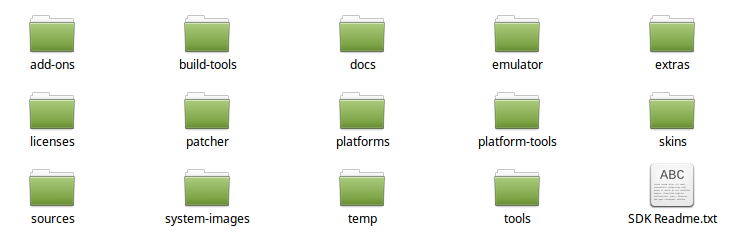
\includegraphics[width=300pt]{img/sdk.png}
}
\frame{
\frametitle{Présentation du SDK android}
\begin{itemize}
  \item add-ons : Google APIs
  \item docs : Copie de la documentation disponible sur d.android.com
  \item extras : Lib de compatibilité, lib pour les achats in-app \ldots
  \item platforms : 1 dossier par niveau d'API téléchargé
  \item platform-tools : Binaires de communication avec les appareils android
  (adb, fastboot \ldots)
  \item samples : Exemples de projets
  \item sources : Sources de chaque niveau d'API
  \item system-images : Images pour l'émulateur
  \item temp
  \item tools : Outils pour le dev (ddms, apkbuilder, lint
  \ldots)
\end{itemize}
}
\frame{
\frametitle{Plugin android pour eclipse : ADT}
\begin{itemize}
  \item Installation comme un plugin eclipse classique
  \item \url{https://dl-ssl.google.com/android/eclipse/}
  \item ADT fait le lien entre eclipse et le SDK android
\end{itemize}
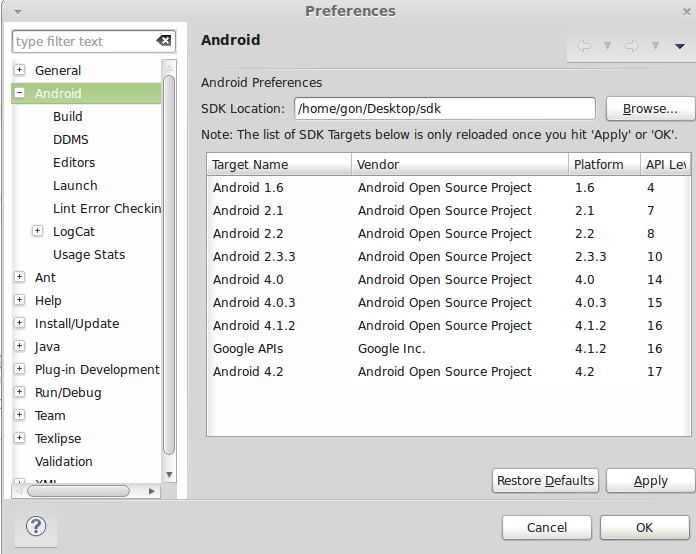
\includegraphics[width=100pt]{img/adt.png}
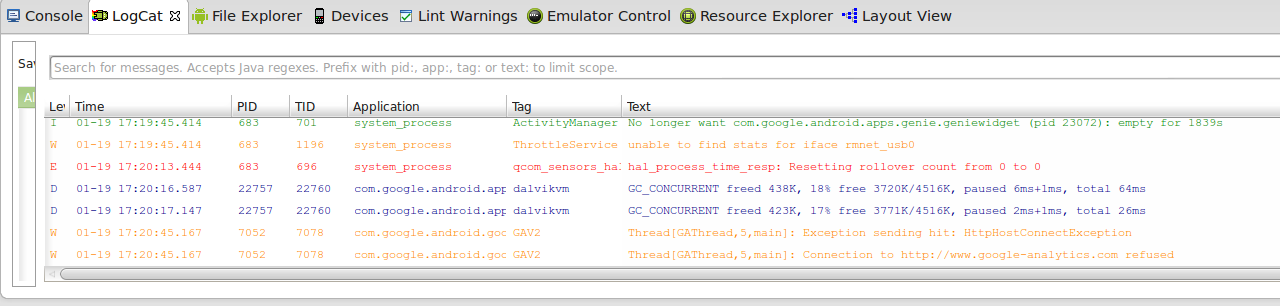
\includegraphics[width=200pt]{img/views.png}\\\\
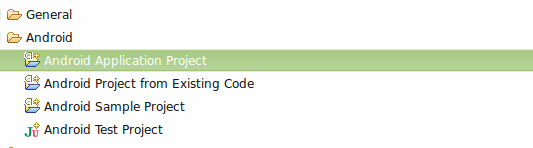
\includegraphics[width=100pt]{img/project.png}
}
\frame{
\frametitle{Android studio}
\begin{itemize}
  \item Basé sur IntelliJ IDEA
  \item IDE retravaillé pour android
  \item IDE officiel depuis décembre 2014
  \item Support natif de gradle
\end{itemize}
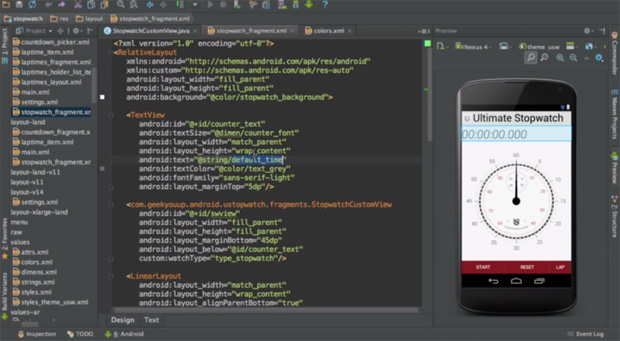
\includegraphics[width=200pt]{img/android-studio.jpg}
}
\frame{
\frametitle{L'émulateur}
\begin{itemize}
  \item Utile pour tester certaines configurations
  \item (très) lent
  \item Utiliser un appareil android à la place quand c'est possible
\end{itemize}
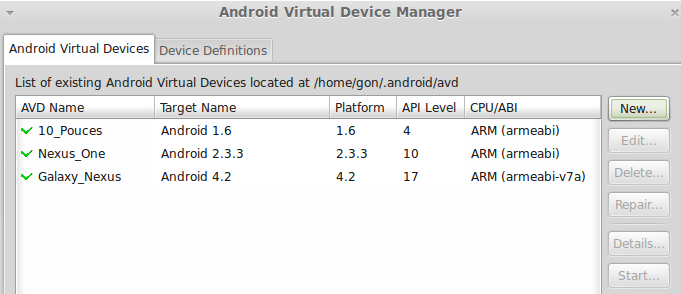
\includegraphics[width=200pt]{img/avd.png}
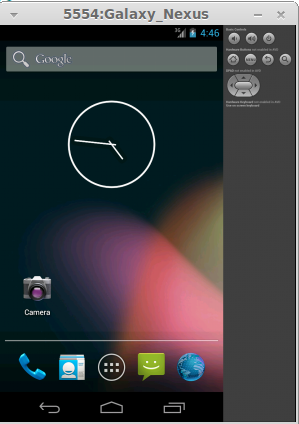
\includegraphics[width=80pt]{img/emu.png}
}
\frame{
\frametitle{Utiliser un appareil android}
\begin{itemize}
  \item Activer les ``options pour les développeurs'' sur l'appareil
  \item Paramètres / A propos du téléphone / Toucher 4 fois ``Numéro de build''
  \item Activer le débogage USB
\end{itemize}
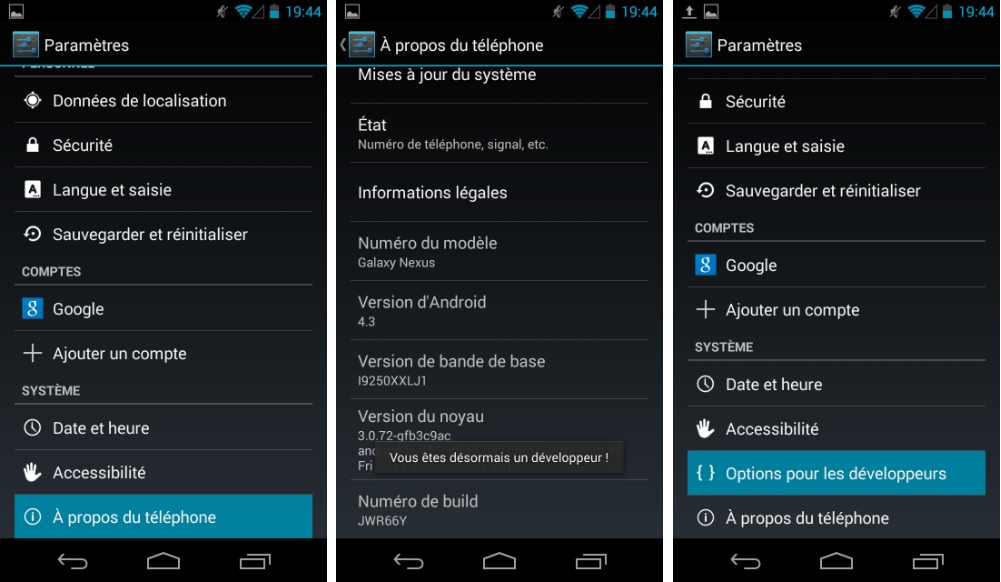
\includegraphics[width=230pt]{img/androiddev.jpg}
}
\subsection{Architecture}
\frame{
\frametitle{Organisation d'un projet android}
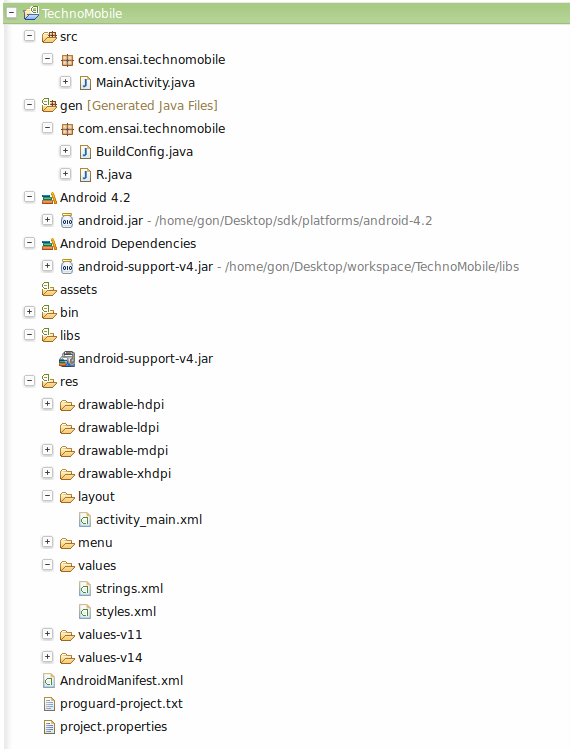
\includegraphics[width=150pt]{img/structure.png}
}
\frame{
\frametitle{Détail de l'organisation}
\begin{itemize}
  \item src : code source Java
  \item gen : identifiants des ressources (généré par le sdk)
  \item Android 4.2 : jar correspondant à l'API cible
  \item Android Dependencies : jar rajoutés, correspond à libs
  \item assets : fichiers fournis avec l'app
  \item bin : résultats des compilations (dont l'apk)
  \item libs : jar rajoutés
  \item res : ressources (layouts, strings, images \ldots)
  \item AndroidManifest.xml : métadonnées sur l'application, composants,
  permissions \ldots
  \item proguard-project.txt : configuration de proguard
  \item project.properties : généré par le sdk
 \end{itemize}
}
\frame{
\frametitle{AndroidManifest.xml : la carte d'identité de l'application}
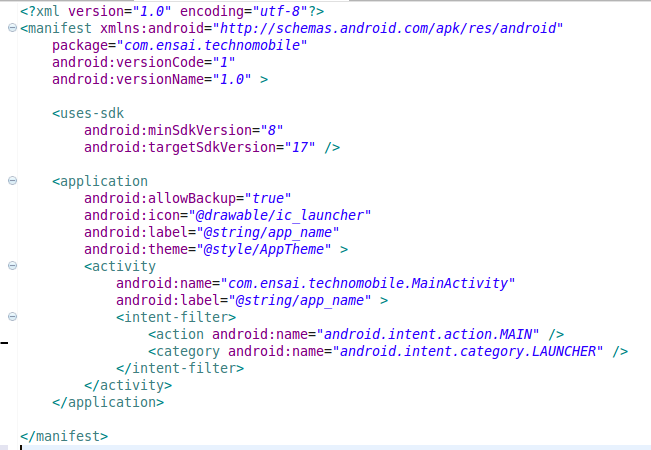
\includegraphics[width=150pt]{img/manifest.png}
\begin{itemize}
  \item Déclaration des composants
  \item Déclaration des permissions
  \item Déclaration d'autres métadonnées de l'application
  \item Analysé par android à l'installation
 \end{itemize}
}
\begin{frame}[fragile]
\frametitle{Les permissions}
\begin{itemize}
  \item Obligatoires pour certaines fonctions (internet, géolocalisation,
  hardware \ldots)
  \item Les applications peuvent définir leurs propres permissions
  \item L'utilisateur est prévenu à l'installation / mise à jour
 \end{itemize}
 \begin{lstlisting}[language=XML]
<uses-permission android:name="android.permission.INTERNET"/>
<uses-permission android:name="android.permission.READ_SMS"/>
<uses-permission android:name="android.permission.CAMERA"/>
\end{lstlisting}
\end{frame} 


\frame{
\frametitle{Le système de ressources}
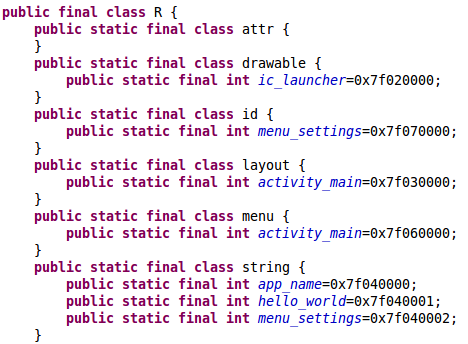
\includegraphics[width=140pt]{img/ressources.png}
\begin{itemize}
  \item Un identifiant est généré pour chaque ressource (drawable, layout, menu,
  values, style \ldots)
  \item Les fonctions qui utilisent des ressources sont surchargées pour aussi
  accepter l'identifiant de la ressource correspondante
  \item Utiliser des ressources différentes en fonction de la configuration
  (values et values-fr, drawable et drawable-hdpi)
   \end{itemize}
}
\begin{frame}[fragile]
\frametitle{Exemple de ressources : les strings}
\begin{itemize}
  \item Eviter au maximum les chaînes de caractères en dur
  \item Mettre toutes les chaînes dans res/values/strings.xml
  \item Très facile de traduire ensuite : res/values-en, res/values-fr \ldots
  (values et values-fr, drawable et drawable-hdpi)
\end{itemize}
\begin{lstlisting}
<resources>
    <string name="app_name">Technomobile</string>
    <string name="hello_world">Hello world!</string>
    <string name="menu_settings">Settings</string>
    <string-array name="statuts">
        <item>Fonctionnaire</item>
        <item>Ingenieur</item>
    </string-array>
</resources>
\end{lstlisting}
\end{frame}
\frame{
\frametitle{Déployer l'application}
\begin{itemize}
  \item Une application android = un APK (+/- équivalent d'un jar)
  \item Une application android doit être signée 
  \item Attention à ne pas perdre la clé !
  \item Création et signature de l'APK simplifié sous eclipse (export)
 \end{itemize}
}
\frame{
\frametitle{Processus de déploiement en développement}
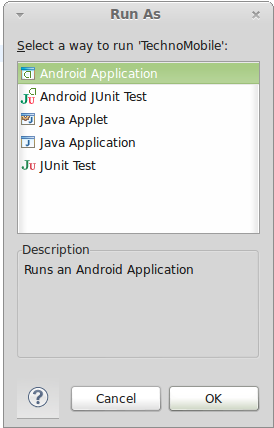
\includegraphics[width=50pt]{img/runas.png}
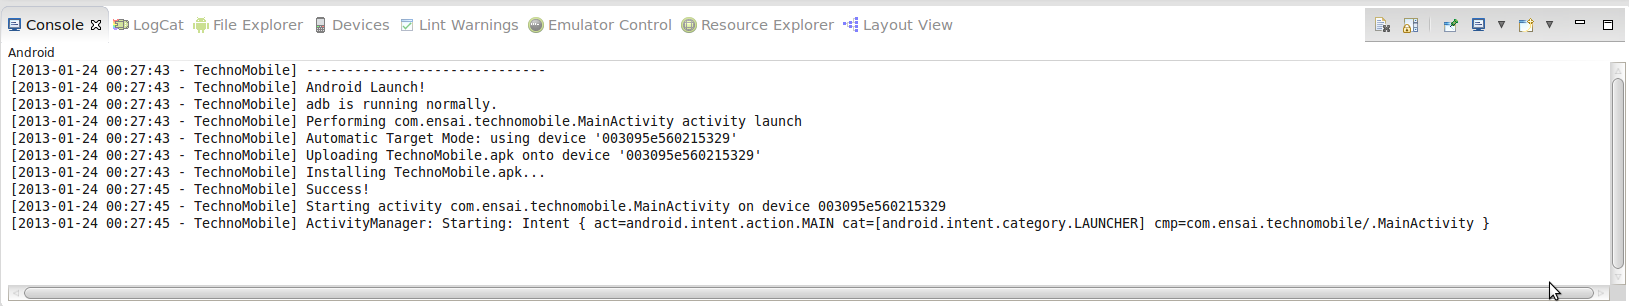
\includegraphics[width=300pt]{img/console.png}
\begin{itemize}
  \item Comme pour une application Java classique, ctrl + F11
  \item Eclipse demande au SDK de builder l'APK
  \item Eclipse signe l'APK avec la clé debug 
  \item Eclipse demande à adb (SDK) d'installer l'application
  \item Soit sur un appareil android connecté soit sur un émulateur
 \end{itemize}
}
\frame{
\frametitle{Distribuer l'application}
\begin{itemize}
  \item Distribution directe de l'APK (ex : pour tester, béta fermée)
  \item Publication sur le playstore, 25\$ à l'inscription
  \item Application gratuite ou payante (30\% pour google)
 \end{itemize}
}
\frame{
\frametitle{Déboguer l'application}
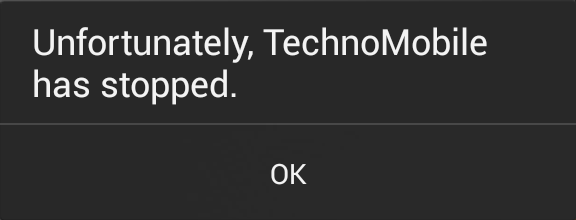
\includegraphics[width=120pt]{img/fc.png}
\begin{itemize}
  \item Si une exception n'est pas rattrapée, android tue l'application
  \item On parle de ``force close'' (FC)
  \item Comment déboguer une application qui tourne sur un appareil (ou
  émulateur) ?
 \end{itemize}
}
\frame{
\frametitle{Logcat, le sauveur}

\includegraphics[width=120pt]{img/logcat.jpg}
\begin{itemize}
  \item Le SDK fournit un outil très pratique : logcat
  \item On appelle logcat par adb : adb logcat ou on utilise la vue LogCat du
  plugin eclipse
  \item Logcat affiche l'ensemble des logs, système et application
 \end{itemize}
}
\frame{
\frametitle{Logcat, exemple}
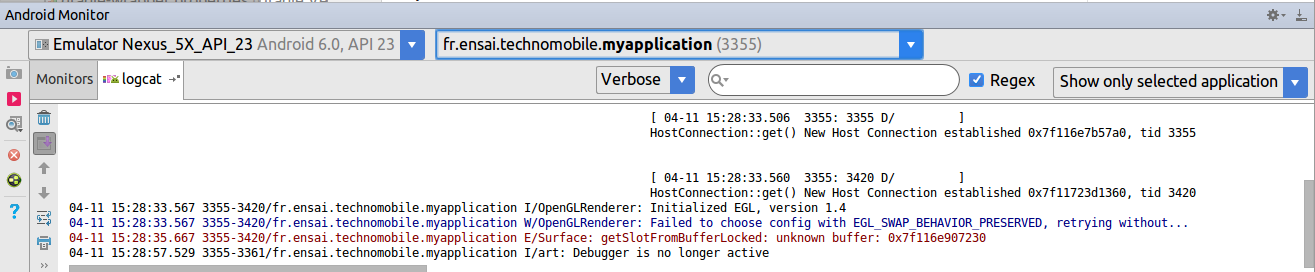
\includegraphics[width=340pt]{img/logeclipse.png}\\
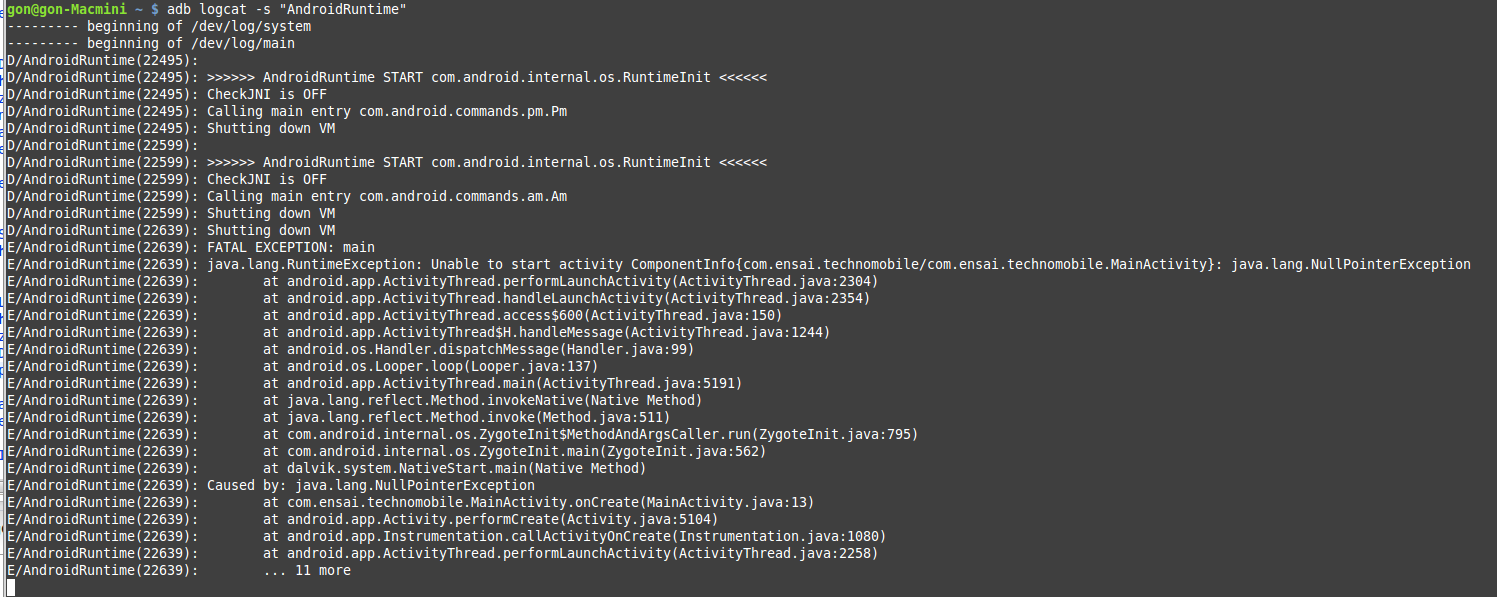
\includegraphics[width=340pt]{img/logterminal.png}
}
\frame{
\frametitle{Stacktrace or GTFO}
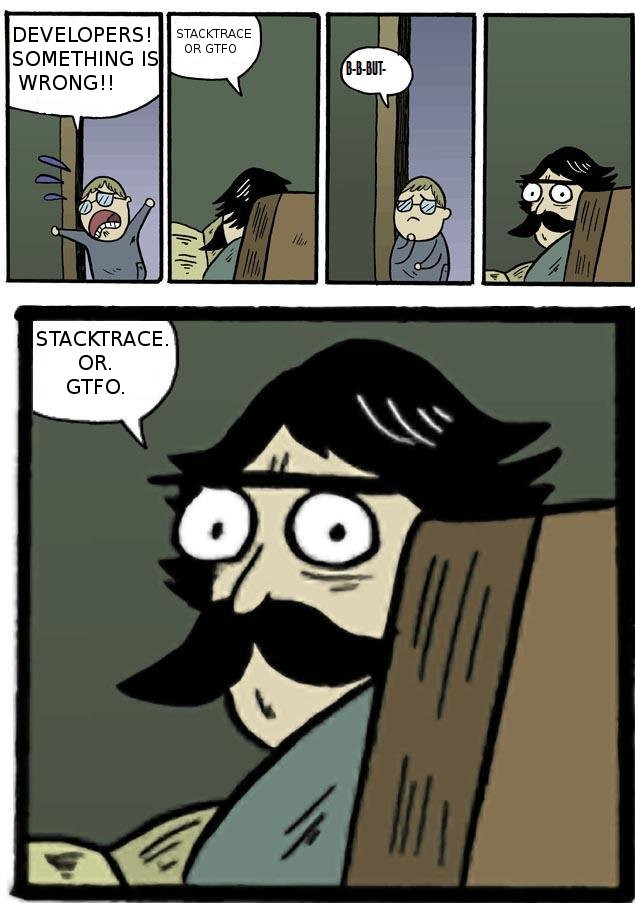
\includegraphics[width=120pt]{img/jacoj.jpg}
}
\begin{frame}[fragile]
\frametitle{Logcat, logging de l'application}
\begin{itemize}
  \item Oublier System.out.println() !
  \item 5 niveaux de gravité : Error, Warn, Info, Debug, Verbose
  \item Possibilité dans adb logcat de filtrer par gravité et/ou TAG
  \item Pratique recommandée : un TAG par application
 \end{itemize}
 \begin{lstlisting}
public void sauvegarderScore(int score) {
        Log.i(TAG,"Sauvegarde du score "+score);
        if (score < 0) {
            Log.w(TAG,"Le score est negatif");
        }
        try {
            //traitement
        }
        catch (Exception e) {
        	Log.e(TAG,"Erreur de score",e);
        }
}
\end{lstlisting}
\end{frame}
\subsection{IHM}
\frame{
\frametitle{Une exécution moins linéaire qu'en Java classique}
\begin{itemize}
  \item Une application android est un ensemble de composants
  \item Pas de méthode main
  \item Des points d'entrée multiples possibles
  \item Exemple : appli SMS
 \end{itemize}
}
\frame{
\frametitle{Activity, le composant de base}
  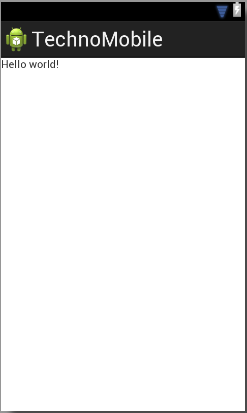
\includegraphics[width=50pt]{img/activity.png}
\begin{itemize}
  \item 1 activity {\raise.17ex\hbox{$\scriptstyle\sim$}}  un écran
  \item Une application peut avoir $0-n$ activities
  \item A déclarer dans le manifest
  \item Créer une classe Java héritant de Activity 
 \end{itemize}
}
\begin{frame}[fragile]
\frametitle{Les Views}
   Une vue = un élément à l'écran
  \begin{itemize}
    \item TextView = Un texte
    \item EditText = Un champ de texte remplissable
    \item ImageView
    \item Button
    \item CheckBox
    \item Plein d'autres views de base dans android
    \item Possibilité de créer ses propres views en héritant (directement ou
    indirectement) de View
 \end{itemize}
\end{frame}
\begin{frame}[fragile]
\frametitle{Les ViewGroups}
  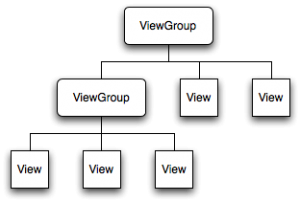
\includegraphics[width=150pt]{img/viewgroup.png}
  \begin{itemize}
 \item LinearLayout
 \item RelativeLayout
 \item ListView
 \item Plein d'autres
 \item Les vôtres
 \end{itemize}
\end{frame}
\begin{frame}[fragile]
\frametitle{L'organisation d'une activity : les layouts} 
\begin{lstlisting}
<LinearLayout 
	xmlns:android="http://schemas.android.com/apk/res/android"
    android:layout_width="match_parent"
    android:layout_height="match_parent">

    <TextView
        android:layout_width="wrap_content"
        android:layout_height="wrap_content"
        android:text="@string/hello_world" />
        
</LinearLayout>
\end{lstlisting}
 \begin{itemize}
  \item Ils définissent l'organisation des vues
 \item Ils sont définis en XML dans le dossier res/layout
 \item @string fait référence à une ressource de strings.xml
 \item Eviter au maximum de modifier / créer les layouts au runtime
 \end{itemize}
\end{frame}
\frame{
\frametitle{Cycle de vie d'une activity} 
  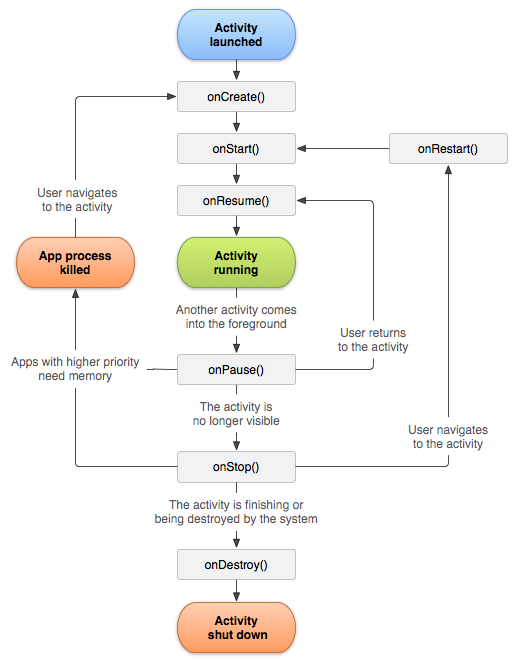
\includegraphics[width=150pt]{img/activity_lifecycle.png}
}
\begin{frame}[fragile]
\frametitle{Créer une activity : étendre Activity} 
\begin{lstlisting}
public Class MainActivity extends Activity {

    @Override
    protected void onCreate(Bundle savedInstanceState) {
        super.onCreate(savedInstanceState);
        setContentView(R.layout.activity_main);
    }
}
\end{lstlisting}
 \begin{itemize}
 \item onCreate est appelé à la création de l'activity (cf cycle de vie)
 \item appel obligatoire à super.onCreate
 \item le bundle savedInstanceState contient les informations en cas de relance
 de l'activity
 \item savedInstanceState est null s'il s'agit du premier lancement
 \end{itemize}
\end{frame}
\begin{frame}[fragile]
\frametitle{Créer une activity : la déclarer dans le manifest} 
\begin{lstlisting}
<activity android:name="com.ensai.technomobile.MainActivity"
          android:label="Accueil" >
    <intent-filter>
        <action android:name="android.intent.action.MAIN" />
        <category android:name="android.intent.category.LAUNCHER" />
    </intent-filter>
</activity>
\end{lstlisting}
 \begin{itemize}
 \item Balise Activity à l'interieur de la balise Application
 \item On précise la classe Java correspondante
 \end{itemize}
\end{frame}
\begin{frame}[fragile]
\frametitle{Manipuler les éléments de l'UI en Java}
Etape 1 : donner un identifiant à la vue
\begin{lstlisting}
<LinearLayout 
	xmlns:android="http://schemas.android.com/apk/res/android"
    android:layout_width="match_parent"
    android:layout_height="match_parent"
    android:id="@+id/monlayout">

    <Button
        android:layout_width="wrap_content"
        android:layout_height="wrap_content"
        android:text="@string/hello_world"
        android:id="@+id/monbouton" />

</LinearLayout>
\end{lstlisting}
\begin{itemize}
    \item @+id crée l'identifiant s'il n'existe pas déjà
    \item L'identifiant doit être unique dans la hiérarchie (sinon conflit)
 \end{itemize}
\end{frame}
\begin{frame}[fragile]
\frametitle{Manipuler les éléments de l'UI en Java}
Etape 2 : récupérer les références vers les views
\begin{lstlisting}
public Class MyActivity extends Activity {

    ViewGroup layout = null;
    Button bouton = null;

    @Override
    protected void onCreate(Bundle savedInstanceState) {
        super.onCreate(savedInstanceState);
        setContentView(R.layout.activity_main);
        layout = (ViewGroup) findViewById(R.id.monlayout);
        bouton = (Button) findViewById(R.id.monbouton);
    }
}
\end{lstlisting}
\begin{itemize}
    \item findViewById renvoie un objet de type View : on cast
    \item si aucune vue n'a l'identifiant demandé, findViewById renvoie null
 \end{itemize}
\end{frame}
\begin{frame}[fragile]
\frametitle{Manipuler les éléments de l'UI en Java}
\begin{lstlisting}
public Class MyActivity extends Activity {
    ViewGroup layout = null;
    Button bouton = null;

    @Override
    protected void onCreate(Bundle savedInstanceState) {
        super.onCreate(savedInstanceState);
        setContentView(R.layout.activity_main);
        layout = (ViewGroup) findViewById(R.id.monlayout);
        bouton = (Button) findViewById(R.id.monbouton);
    }
	
    public void changerTexte(String texte) {
        bouton.setText(texte);
    }
	
    public void cacherTout() {
        layout.setVisibility(View.INVISIBLE);
    }
}
\end{lstlisting}
\end{frame}
\begin{frame}[fragile]
\frametitle{Ecouter les événements}
\begin{itemize}
 \item Système de listeners (cf swing)
 \item Il se passe quelque chose sur la vue (touch, focus \ldots) : le listener
 est prévenu
 \item Pour simplifier, sur android on n'a en général qu'un listener par
 événement et par view (setXListener au lieu de addXListener sous swing)
 \end{itemize}
\end{frame}
\begin{frame}[fragile]
\frametitle{Ecouter les événements, guide du bon listener}
Etape 1 : Les interfaces XListener (elles existent déjà, ne pas les réécrire !)
\begin{lstlisting}
public Interface OnClickListener {
    public void onClick(View v);
}
\end{lstlisting}
Etape 2 : Implémenter l'interface
\begin{lstlisting}
public MaClasse implements OnClickListener {
    public void onClick(View v) {
        //Un click a ete fait sur la vue v
    }
}
\end{lstlisting}
\end{frame}
\begin{frame}[fragile]
\frametitle{Ecouter les événements, guide du bon listener}
Etape 3 : S'enregistrer comme listener
\begin{lstlisting}
public Class MyActivity extends Activity implements OnClickListener {

    Button bouton = null;

    @Override
    protected void onCreate(Bundle savedInstanceState) {
        super.onCreate(savedInstanceState);
        setContentView(R.layout.activity_main);
        bouton = (Button) findViewById(R.id.monbouton);
        bouton.setOnClickListener(this);
    }
	
    public void onClick(View v) {
        //Un Click a ete fait sur la vue v
    }
}
\end{lstlisting}
\end{frame}
\begin{frame}[fragile]
\frametitle{Ecouter les événements, quelques feintes}
Feinte 1 : Utiliser des listeners anonymes
\begin{lstlisting}
public Class MyActivity extends Activity implements OnClickListener {

    Button bouton = null;

    @Override
    protected void onCreate(Bundle savedInstanceState) {
        super.onCreate(savedInstanceState);
        setContentView(R.layout.activity_main);
        bouton = (Button) findViewById(R.id.monbouton);
        bouton.setOnClickListener(new OnClickListener() {
                public void onClick(View v) {
                //Un Click a ete fait sur la vue v
                }
            });
	    }
}
\end{lstlisting}
\end{frame}
\begin{frame}[fragile]
\frametitle{Ecouter les événements, quelques feintes}
Feinte 2 : Définir le listener directement dans le layout
\begin{lstlisting}
<LinearLayout 
	xmlns:android="http://schemas.android.com/apk/res/android"
    android:layout_width="match_parent"
    android:layout_height="match_parent"
    android:id="@+id/monlayout">

    <Button
        android:layout_width="wrap_content"
        android:layout_height="wrap_content"
        android:id="@+id/monbouton"
        android:text="@string/hello_world"
        android:onClick="clickSurLeBouton" />

</LinearLayout>
\end{lstlisting}
\begin{lstlisting}
public void clickSurLeBouton(View v) //dans MyActivity
\end{lstlisting}
\end{frame}

\begin{frame}[fragile]
\frametitle{La classe abstraite context}
\begin{itemize}
 \item La plupart des fonctions d'android (accéder à une ressource,
 lancer une activité \ldots) nécessitent une instance de Context
 \item Un Context regroupe des informations globales sur l'environnement de
 l'application
 \item Android se charge de créer les contextes, n'en instanciez pas !
 \item Activity hérite (indirectement) de Context
 \item Les views ont toutes une réference vers un context
 \end{itemize}
\end{frame}

\begin{frame}[fragile]
\frametitle{Affichage d'un court message : le toast}
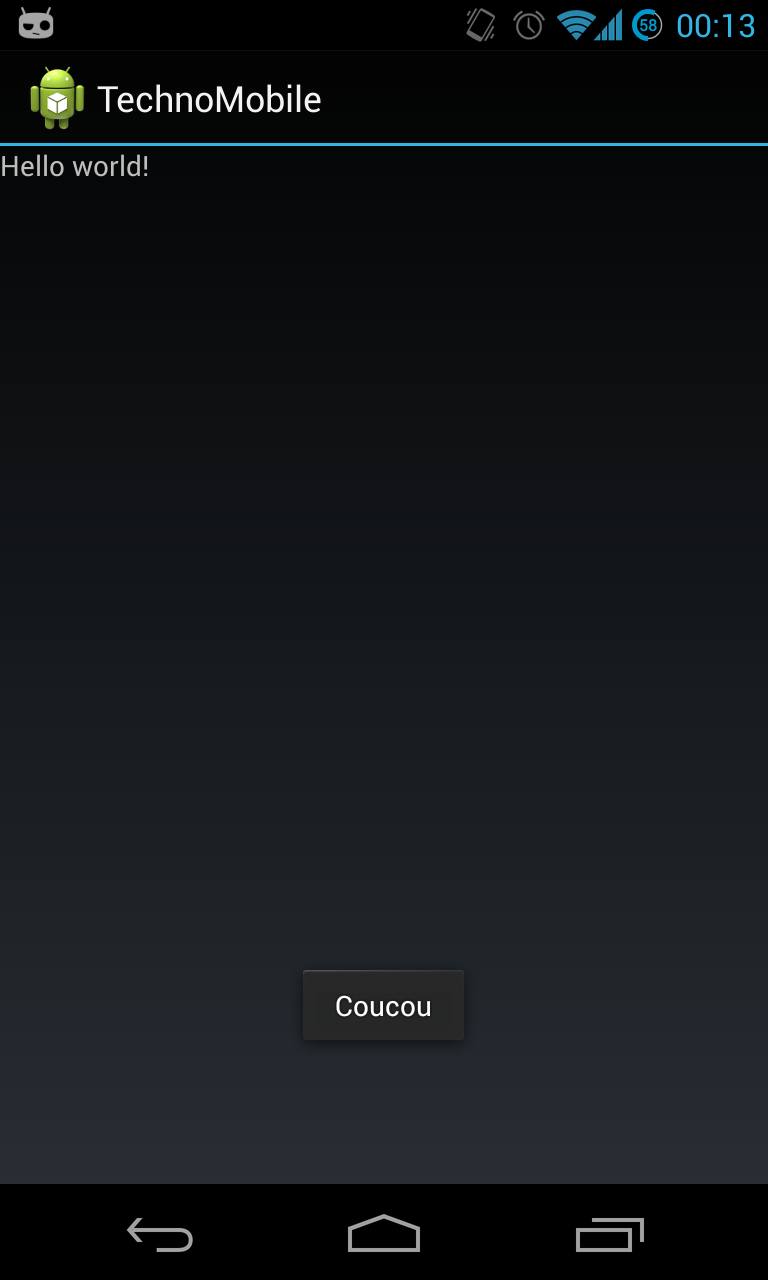
\includegraphics[width=60pt]{img/coucou.png}
\begin{lstlisting}
public MyActivity extends Activity {
    
    public void faireCoucou() {
        Toast.makeText(this,"Coucou",Toast.LENGTH_LONG).show();
        Toast.makeText(this,R.string.coucou,Toast.LENGTH_SHORT).show();
    }	
}
\end{lstlisting}
\end{frame}
\begin{frame}[fragile] 
\frametitle{Previously on Android}
\begin{itemize}
  \item Une appli = un ensemble de composants
  \item Plusieurs points d'entrée possibles
  \item Tous les composants doivent être définis dans le manifest
  \item Activity, composant {\raise.17ex\hbox{$\scriptstyle\sim$}} un écran
  \item Créer une activity = hériter de Activity
  \item Méthodes du cycle de vie (onCreate, onPause, onResume \ldots)
\end{itemize}
\end{frame}
\begin{frame}[fragile] 
\frametitle{Previously on Android, les layouts}
\begin{itemize}
  \item Les composants graphiques sont définis dans des layouts XML
  \item Layout = hiérarchie de ViewGroup et de View
  \item Exemple de ViewGroup : LinearLayout
  \item Exemples de View : Button, TextView, EditText
  \item Tous les élements doivent définir layout\_width et layout\_height
  \item Wrap\_content : seulement la place nécessaire
  \item Match\_parent : toute la place du père
  \item Plaquer (inflate) un layout à une activity :
  setContentView(R.layout.xxx)
\end{itemize}
\end{frame}
\begin{frame}[fragile] 
\frametitle{Previously on Android, manipuler les élements UI}
\begin{itemize}
  \item Pour manipuler les éléments UI en Java : leur donner un ID
  \item @+id/identifiant : crée un int IDENTIFIANT dans R.id
  \item R : fichier autogénéré des ressources
  \item Dans l'activity : utiliser findViewById(R.id.identifiant)
  \item Caster la valeur trouvée
  \item Ensuite, usage classique : bouton.setText(\ldots)
\end{itemize}
\end{frame}
\begin{frame}[fragile] 
\frametitle{Previously on Android, écouter les évenements}
\begin{itemize}
  \item Implémenter OnXListener (ex : OnClickListener)
  \item S'enregistrer comme listener auprès de la View
  (ex : bouton.setOnClickListener(\ldots))
  \item Chaque événement correspond à un appel de la méthode implémentée
  \item Feinte 1 : enregistrer des listeners anonymes (créés ad-hoc)
  \item Feinte 2 : déclarer le listener dans le layout XML (View onClick)
  
\end{itemize}
\end{frame}
\begin{frame}[fragile]
\frametitle{Les autres composants d'une application : les services}
\begin{itemize}
 \item Tâche en arrière plan
 \item Cycle de vie différent de celui d'une activity
 \item Pas d'interface graphique (sauf si une activity communique avec le
 service)
 \item Exemples : lecteur MP3, client torrent, système de mise à jour, taskkiller \ldots
 \end{itemize}
\end{frame}
\begin{frame}[fragile]
\frametitle{Les autres composants d'une application : les broadcast receivers}
\begin{itemize}
 \item Composant recevant les annonces système et les annonces des autres applications
 \item Permet de réagir à certains événements
 \item Possibilité de lancer des activités ou des services depuis le broadcast receiver
 \item Exemples : indicateur de batterie, antivirus, lancement au démarrage,
 intercepter un appel ou un SMS reçu \ldots
 \end{itemize}
\end{frame}
\begin{frame}[fragile]
\frametitle{Les autres composants d'une application : les content-providers}
\begin{itemize}
  \item Composant servant à distribuer les données
  \item Peu importe comment les données sont stockées (sqlite, préférences, fichier \ldots)
  \item Respecte une interface d'utilisation des données
  \item Peut permettre la récupération, la modification et/ou la suppression de données
  \item Principalement destiné à une utilisation entre applications
  \item Gestion de la sécurité et des droits (permissions)
  \item Exemple : accès aux données système (SMS, contacts \ldots) 
 \end{itemize}
\end{frame}

\begin{frame}[fragile]
\frametitle{Les intents}
\begin{itemize}
 \item Messages asynchrones échangés entre applications ou entre composants
 \item On déclare son intention, android réagit en conséquence
 \end{itemize}
Un intent est constitué de plusieurs informations principales :
\begin{itemize}
 \item action : l'action à effectuer 
 \item data : les données concernées, sous la forme d'une URI
 \item Ex : ACTION\_VIEW content://contacts/people/1
 \item ACTION\_DIAL tel:123
 \end{itemize}
Et d'informations secondaires : 
\begin{itemize}
 \item category : pour préciser l'action
 \item type : pour forcer le type de données 
 \item extras : des données libres supplémentaires
 \item component : dans le cas des intents explicites
 \end{itemize}
\end{frame}
\begin{frame}[fragile]
\frametitle{Lancer un intent implicite}
``Je veux envoyer un mail à annee2@ensai.fr avec le titre URGENT : FOOT''
\begin{lstlisting}
public MyActivity extends Activity {
    
    public void envoyerMail() {
        Intent i = new Intent(Intent.ACTION_SEND);
        i.setType("message/rfc822");
        i.putExtra(Intent.EXTRA_EMAIL  , "annee2@ensai.fr");
        i.putExtra(Intent.EXTRA_SUBJECT,"URGENT : FOOT"); 
        i.putExtra(Intent.EXTRA_TEXT   , "...");
        try {
            startActivity(i);
        } 
        catch (ActivityNotFoundException ex) {
            //Pas de client mail installe
        }
    }	
}
\end{lstlisting}
\end{frame}
\begin{frame}[fragile]
\frametitle{Lancer un intent explicite}
``Je veux lancer l'activity ProfilActivity en transmettant l'id 42''
\begin{lstlisting}
public MyActivity extends Activity {
    public void visualiserProfil() {
        Intent intent = new Intent(this, ProfilActivity.class); 
        //this est la en tant que context
        intent.putExtra("id",42);
        startActivity(intent);
    }	
}
\end{lstlisting}

\begin{lstlisting}
public ProfilActivity extends Activity {
    protected void onCreate(Bundle savedInstanceState) {
        super.onCreate(savedInstanceState);
        Intent intent = getIntent();
        int id = intent.getIntExtra("id",-1);
    }
}
\end{lstlisting}
\end{frame}

\begin{frame}[fragile]
\frametitle{Filtrer les intents, le principe}
\begin{itemize}
    \item startActivity(), startService() et sendBroadcast() déclenchent des
    intents
	\item android filtre les composants susceptibles de recevoir l'intent en
	fonction à partir des intent-filters de chaque composant
\end{itemize}

\begin{lstlisting}
<activity android:name="com.ensai.technomobile.MainActivity"
            android:label="@string/app_name" >
            <intent-filter>
                <action android:name="android.intent.action.MAIN" />
                <category android:name="android.intent.category.LAUNCHER" />
            </intent-filter>
        </activity>
\end{lstlisting}
\end{frame}
\begin{frame}[fragile]
\frametitle{Filtrer les intents, exemple}
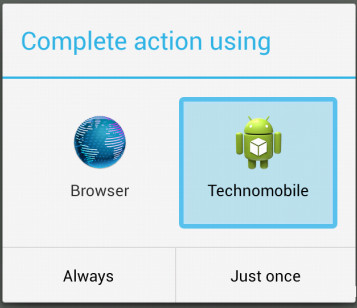
\includegraphics[width=45pt]{img/intentchooser.jpg}
\begin{lstlisting}
<activity
            android:name="com.ensai.technomobile.TwitterActivity"
            android:label="@string/app_name" >
            <intent-filter>
                <data
                    android:host="twitter.com"
                    android:scheme="http" />
                <category android:name="android.intent.category.DEFAULT" />
                <category android:name="android.intent.category.BROWSABLE" />
                <action android:name="android.intent.action.VIEW" />
            </intent-filter>
        </activity>
\end{lstlisting}
\end{frame}

\subsection{Les données}
\frametitle{Gestion des données}
\begin{frame}
Il existe plusieurs façons de stocker les données sur un appareil android
\begin{itemize}
    \item \textbf{SharedPreferences}: stockage de données primitives
    \item \textbf{Fichiers}: contenus sur la mémoire interne ou externe
    \item \textbf{Bases de données}: SQLite
    \item \textbf{Stockage distant}: webservice
\end{itemize}
Documentation android officielle sur le stockage de données : \url{http://developer.android.com/guide/topics/data/data-storage.html}
\end{frame}

\begin{frame}
\frametitle{SharedPreferences}
\begin{itemize}
    \item Equivalent des Preferences de Java
    \item Stockage de données primitives (int, boolean, String \ldots)
    \item Mapping clé / valeur
    \item Très facile de créer un écran de paramètres (PreferenceActivity)
    \item Système de listeners pour être prévenu lors d'un changement
    \item Léger à implémenter
\end{itemize}
\end{frame}
\begin{frame}[fragile]
\frametitle{SharedPreferences, accéder aux préférences}
Accéder simplement aux préférences :\\
\begin{lstlisting}
public void sauvegarderScore() {
    SharedPreferences preferences = PreferenceManager.getDefaultPreferences(context);
}
\end{lstlisting}
Accéder en précisant le nom et le mode :\\
\begin{lstlisting}
public void sauvegarderScore() {
    SharedPreferences preferences = context.getSharedPreferences("toto",Context.MODE_PRIVATE);
}
\end{lstlisting}
L'utilisation d'autres modes que MODE\_PRIVATE est découragé depuis l'API 17 (4.2) pour des raisons de sécurité.\\
\end{frame}
\begin{frame}[fragile]
\frametitle{SharedPreferences, utilisation des préférences}
Lire les préférences :\\
\begin{lstlisting}
public void afficherMeilleurScore() {
    SharedPreferences preferences = PreferenceManager.getDefaultPreferences(context);
    int record = preferences.getInt("meilleurScore");
    Toast.makeText(context, "Record : "+record,Toast.LENGTH_LONG).show();
}
\end{lstlisting}
Modifier les préférences\\
\begin{lstlisting}
public void sauvegarderScore() {
    SharedPreferences preferences = PreferenceManager.getDefaultPreferences(context);
    Editor editor = preferences.edit();
    editor.putInt("meilleurScore",42);
    editor.commit();
}
\end{lstlisting}
\end{frame}
\begin{frame}[fragile]
\frametitle{Les fichiers}
\begin{itemize}
    \item API classiques de Java (File, InputStream, OutputStream \ldots)
    \item Ne jamais utiliser de chemin absolu, utiliser les fonctions android pour déterminer les dossiers
    \item Garder en tête les contraintes du mobile : espace libre, SD accessible
    \item Choisir entre stockage interne et externe
\end{itemize}
\end{frame}
\begin{frame}[fragile]
\frametitle{Stockage interne}
\begin{lstlisting}
FileOutputStream fos = context.openFileOutput("monFichier.ext", Context.MODE_PRIVATE);
fos.write("texte".getBytes());
fos.close();
\end{lstlisting}
\begin{itemize}
    \item Comme pour les préférences, ne pas utiliser les modes WORLD\_READABLE et WORLD\_WRITEABLE
    \item Les fichiers créés sur le stockage interne sont liés à l'application
    (en particulier, ils sont supprimés lors de la désinstallation de l'application)
\end{itemize}
\begin{itemize}
    \item getCacheDir() : répertoire pour le cache
    \item getFilesDir() : dossier des fichiers de l'application
    \item deleteFile(String nom)
    \item fileList() : String[] des fichiers créés par l'application
\end{itemize}
\end{frame}
\begin{frame}[fragile]
\frametitle{Stockage externe}
\begin{itemize}
    \item La jungle : l'utilisateur et toutes les applications peuvent lire / écrire tout le contenu
    \item La présence d'un stockage externe n'est pas garanti
    \item Même s'il est présent, le stockage externe peut ne pas être
    disponible (appareil connecté au PC)
    \item 2 permissions : WRITE\_EXTERNAL\_STORAGE et READ\_EXTERNAL\_STORAGE
\end{itemize}
\begin{lstlisting}
String state = Environment.getExternalStorageState();
if (Environment.MEDIA_MOUNTED.equals(state)) {
    //Lecture et ecriture possibles
} 
else if (Environment.MEDIA_MOUNTED_READ_ONLY.equals(state)) {
    //Lecture possible, ecriture impossible
} 
else { //Lecture et ecriture impossibles }
\end{lstlisting}
\end{frame}
\begin{frame}[fragile]
\frametitle{Stockage externe, utilisation}
Pour le contenu utilisé uniquement par l'application :
\begin{lstlisting}
File file = new File(getExternalFilesDir(null), "DemoFile.jpg");
\end{lstlisting}
Ces fichiers seront supprimés lors de la désinstallation de l'application\\\\
Pour le contenu destiné à être partagé (donc persistant même après une
désinstallation) :
\begin{lstlisting}
File file = new File(getExternalStoragePublicDirectory(Environment.DIRECTORY_PICTURES), "DemoFile.jpg");
\end{lstlisting}
L'argument utilisé dans les 2 cas correspond au type de données et est une variable static de Environment\\
Exemples : Environment.DIRECTORY\_PICTURES, DIRECTORY\_MUSIC, DIRECTORY\_DOWNLOADS, DIRECTORY\_DCIM \ldots
\end{frame}
\begin{frame}[fragile]
\frametitle{SQLite, le moteur de base de données portable}
\begin{itemize}
    \item SQLite est un moteur de base de données spécialement conçu pour le
    mobile et l'embarqué
    \item On retrouve à peu près l'ensemble des fonctions de base d'un moteur de BDD
    \item Android propose en plus une API facilitant les tâches courantes : SQLiteOpenHelper
    \item Pour les requêtes, android offre une API proche de JDBC
\end{itemize}
\end{frame}
\begin{frame}[fragile]
\frametitle{Mise en place d'une base de données SQLite}
Etape 1 : étendre SQLiteOpenHelper 
\begin{lstlisting}
public class MyOpenHelper extends SQLiteOpenHelper {

    private static final int DATABASE_VERSION = 1;
    private static final String DATABASE_NAME = "mabase";

    public MyOpenHelper(Context context) {
        super(context, DATABASE_NAME, null, DATABASE_VERSION);
    }
}
\end{lstlisting}
Etape 2 : implémenter onCreate
\begin{lstlisting}
    @Override
    public void onCreate(SQLiteDatabase db) {
       db.execSQL("CREATE TABLE exemple (nom TEXT PRIMARY KEY, score INTEGER)");
       }
\end{lstlisting}
\end{frame}
\begin{frame}[fragile]
\frametitle{Mise en place d'une base de données SQLite}
Etape 3 : Organiser les mises à jour de la base
\begin{lstlisting}
public class MyOpenHelper extends SQLiteOpenHelper {
    @Override
    public void onUpgrade(SQLiteDatabase db, int oldVersion, int newVersion) {
        //Mise a jour de la base si besoin
    }
}
\end{lstlisting}
\begin{itemize}
    \item L'entier DATABASE\_VERSION permet de savoir si une mise à jour de la base est nécessaire
    \item Android appelle directement onUpgrade si le numéro de version est supérieur au numéro de version actuel de la base
    \item onUpgrade doit alors faire les mises à jour qui s'imposent en fonction
    des entiers oldVersion / newVersion
\end{itemize}
\end{frame}
\begin{frame}[fragile]
\frametitle{Utilisation de SQLite}
Récupérer une instance de SQLiteDatabase
\begin{lstlisting}
SQLiteOpenHelper helper = new SQLiteOpenHelper(context);
SQLiteDatabase writableDB = helper.getWritableDatabase();
SQLiteDatabase readableDB = helper.getReadableDatabase();
\end{lstlisting}
\begin{itemize}
    \item Android propose un certain nombre de fonctions utilitaires pour le
    requêtage, l'insertion, la mise à jour et la suppression de données
    \item Penser à fermer la base avec .close() pour libérer des ressources
\end{itemize}
\end{frame}
\begin{frame}[fragile]
\frametitle{Utilisation de SQLite, les requêtes}
\begin{itemize}
    \item 2 méthodes au choix en fonction du besoin
    \item Ces méthodes sont déclinées en de multiples méthodes (surcharge)
    \item rawQuery(String sql, String[] selectionArgs) pour du sql dur ({\raise.17ex\hbox{$\scriptstyle\sim$}} PreparedStatement)
    \item query(String table, String[] columns, String selection, String[] selectionArgs, String groupBy, String having, String orderBy) pour que android génère le sql
\end{itemize}
\begin{lstlisting}
SQLiteDatabase writableDB = helper.getWritableDatabase();
Cursor cursor1 = writableDB.rawQuery("SELECT nom,score FROM table WHERE id =?",new String[] {"1"}); 
Cursor cursor2 = writableDB.query("table",new String[] {"nom","score"}, "id =?",new String[] {"1"}, null, null, null );
\end{lstlisting}
\end{frame}
\begin{frame}[fragile]
\frametitle{Utilisation de SQLite, les cursors}
\begin{itemize}
    \item Wrapper autour d'un ResultSet
    \item Utilisation très proche des resultSets
    \item Penser à le fermer (close()) pour libérer des ressources
\end{itemize}
\begin{lstlisting}
int nbRows = cursor.getCount();
while (cursor.moveToNext()) {
    String nom = cursor.getString(0);
    int score = cursor.getInt(1);
}
cursor.close();
\end{lstlisting}
\end{frame}
\begin{frame}[fragile]
\frametitle{Utilisation de SQLite : update, insert et delete}
long insert (String table, String nullColumnHack, ContentValues values)
\begin{lstlisting}
ContentValues values = new ContentValues();
values.put("nom", "Bob");
values.put("score", 42);
long rowID = bdd.insert(table, null, values);
\end{lstlisting}
int update(String table, ContentValues values, String whereClause, String[] whereArgs)
\begin{lstlisting}
ContentValues values = new ContentValues();
values.put("score", 43);
int nbRowsAffected = bdd.update(table, values, "nom = ?",new String[] {"Bob"});
\end{lstlisting}
int delete (String table, String whereClause, String[] whereArgs)
\begin{lstlisting}
int nbRowsAffected = bdd.delete(table,"nom = ?", new String[] {"Bob"});
\end{lstlisting}
\end{frame}
\subsection{Bonus}
\begin{frame}[fragile]
\frametitle{La propriété Layout\_weight de LinearLayout}
\begin{itemize}
  \item Possibilité d'assigner des ``importances'' aux views d'un LinearLayout
  \item Attribut layout\_weight défini dans les fils
  \item Les views occupent l'espace restant au prorata de leur importance
  \item Si layout\_weight n'est pas défini, il vaut 0
\end{itemize}
\end{frame}
\begin{frame}[fragile]
\frametitle{La propriété Layout\_weight de LinearLayout, exemple}
\begin{lstlisting}
<LinearLayout xmlns:android="http://schemas.android.com/apk/res/android"
    android:layout_width="match_parent"
    android:layout_height="match_parent" >
    <Button
        android:layout_width="wrap_content"
        android:layout_height="wrap_content"
        android:text="1"
        android:layout_weight="1" />
    <Button
        android:layout_width="wrap_content"
        android:layout_height="wrap_content"
        android:text="2"
        android:layout_weight="2" />
    <Button
        android:layout_width="wrap_content"
        android:layout_height="wrap_content"
        android:text="3" />
</LinearLayout> 
\end{lstlisting}
\end{frame}
\begin{frame}[fragile]
\frametitle{La propriété Layout\_weight de LinearLayout, résultat}
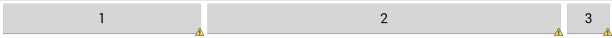
\includegraphics[width=330pt]{img/weight.png}
\begin{itemize}
  \item Toutes les vues prennent la place dont elles ont besoin
  \item On calcule la place restante
  \item On répartit au prorata des poids
  \item Exemple notable : si une seule vue a un poids, elle prend toute la place
  restante
\end{itemize}
\end{frame}
\begin{frame}[fragile]
\frametitle{Exemples de ViewGroups : RelativeLayout}
Plus évolué que LinearLayout, permet de placer les composants les uns par rapport aux autres
\begin{lstlisting}
<RelativeLayout xmlns:android="http://schemas.android.com/apk/res/android"
    android:layout_width="match_parent"
    android:layout_height="match_parent" >
    <EditText
    	android:id="@+id/text1"
        android:layout_width="wrap_content"
        android:layout_height="wrap_content"
        android:layout_alignParentLeft="true"
        android:layout_alignParentTop="true" />
    <Button
        android:layout_width="wrap_content"
        android:layout_height="wrap_content"
        android:layout_alignParentLeft="true"
        android:layout_below="@+id/text1" />
</RelativeLayout> 
\end{lstlisting}
\end{frame}
\begin{frame}[fragile]
\frametitle{Exemples de ViewGroups : ScrollView}
Englobe une view et affiche une scroll bar si la view est trop grande
\begin{lstlisting}
<ScrollView xmlns:android="http://schemas.android.com/apk/res/android"
    android:layout_width="match_parent"
    android:layout_height="match_parent"
    android:orientation="vertical" >
    <TextView
        android:id="@+id/TextView01"
        android:layout_width="wrap_content"
        android:layout_height="wrap_content"
        android:text="@string/longlonglongtexte" >
    </TextView>
</ScrollView> 
\end{lstlisting}
\end{frame}
\begin{frame}[fragile]
\frametitle{Exemples de ViewGroups : ListView}
\begin{itemize}
  \item Pattern ultra classique des applications mobile
  \item Affichage d'un nombre variable d'éléments avec, si besoin, une scroll bar
  \item Récupération des events (press, longpress \ldots) sur les éléments de la liste
  \item Chaque élement est affiché dans une view différente à l'intérieur de la listview
\end{itemize}
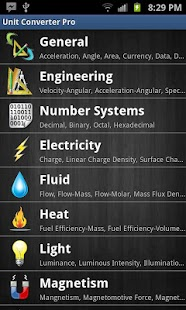
\includegraphics[width=80pt]{img/listview.jpg}
\end{frame}
\begin{frame}[fragile]
\frametitle{ListView : les adapters}
\begin{itemize}
  \item Les adapters font le lien entre les données et l'affichage (view) 
  \item Un adapter hérite de BaseAdapter
  \item 2 implémentations classiques : 
  \item ArrayAdapter pour les données sous forme d'array / list
  \item (Simple)CursorAdapter pour les données sous forme de Cursor
\end{itemize}
Extrait de la classe abstraite BaseAdapter :
\begin{lstlisting}
public abstract View getView(int position, View convertView, ViewGroup parent);
public abstract long getItemId(int position);
public abstract Object getItem(int position);
public abstract int getCount();
\end{lstlisting}
\end{frame}
\begin{frame}[fragile]
\frametitle{ListView : exemple d'utilisation d'ArrayAdapter}
\begin{lstlisting}
ListView listView = (ListView) findViewById(R.id.mylist);
String[] values = { "ligne1","ligne2","ligne3"};

// 1) Context
// 2) Layout a utiliser pour chaque view
// 3) ID de la textview a l'interieur du layout 
//(optionnel, par defaut : android.R.id.text1) 
// 4) Liste / tableau des donnees
ArrayAdapter<String> adapter = new ArrayAdapter<String>(this,
  android.R.layout.simple_list_item_1, android.R.id.text1, values);

listView.setAdapter(adapter); 
//Manipulation des donnees
adapter.add("ligne 4");
adapter.clear();
\end{lstlisting}
\end{frame}
\begin{frame}[fragile]
\frametitle{ListView : écouter les événements}
Les événements comme les clicks sont gérés par la listview (et non pas par l'adapter)
\begin{lstlisting}
listView.setOnItemClickListener(new OnItemClickListener() {
  public void onItemClick(AdapterView<?> parent, View view,
    int position, long id) {
    //position, id et view concernes 
    //parent == listview
  }
});
\end{lstlisting}
\end{frame}
\begin{frame}[fragile]
\frametitle{Créer sa propre view}
\begin{itemize}
  \item Dans certains cas, les views de base d'android ne suffisent pas
  \item Exemple : création d'un jeu, création d'un color picker \ldots
  \item On peut alors chercher si d'autres développeurs n'ont pas déjà créé des
  views semblables
  \item ex : \url{http://androidviews.net}, \url{http://google.fr}
  \item ou créer ses propres views en héritant de View ou SurfaceView
  \item View : view classique, rafraichissement au besoin
  \item SurfaceView : view ``temps réel'' (pour un jeu par exemple)
\end{itemize}
\end{frame}
\begin{frame}[fragile]
\frametitle{Créer sa propre view}
Etape 1 : hériter de View
\begin{lstlisting}
public class CustomView extends View {

    public CustomView(Context context) {
        super(context);
    }
    
    public CustomView(Context context, AttributeSet attrs) {
        super(context, attrs);
    }

    public CustomView(Context context, AttributeSet attrs, int defStyle) {
        super(context, attrs, defStyle);
    }
   
}
 \end{lstlisting}
\end{frame}
\begin{frame}[fragile]
\frametitle{Créer sa propre view}
Etape 2 : implémenter onDraw
\begin{lstlisting}
public class CustomView extends View {

    @Override
    protected void onDraw(Canvas canvas) {
        super.onDraw(canvas);
        canvas.drawColor(Color.BLUE);
        int largeur = canvas.getWidth();
        int hauteur = canvas.getHeight();
        //canvas.drawString
        //canvas.drawCircle
        //canvas.drawBitmap
    }
}
\end{lstlisting}
\end{frame}
\begin{frame}[fragile]
\frametitle{Previously on Android, S01E02}
\begin{itemize}
  \item Une application = un ensemble de composants définis dans le manifest
  \item Composants = Activity, Service, BroadcastReceiver, ContentProvider
  \item L'organisation des views pour l'interface graphique se fait en XML dans
  les fichiers layout
  \item Manipuler des views = leur donner un identifiant et appeler findViewById
\end{itemize}
\end{frame}
\begin{frame}[fragile]
\frametitle{Previously on Android, S01E02}
\begin{itemize}
  \item Intents = messages inter-composants / inter-applications
  \item Intent implicite = une action à faire (ex : envoyer un mail, afficher
  les contacts), android cherche les composants capables de répondre
  \item Android filtre en fonction des intent-filters définis dans le manifest
  \item Intent explicite = on invoque un composant particulier
  \item Les intents peuvent avoir des données ``Extra''
\end{itemize}
\end{frame}
\begin{frame}[fragile]
\frametitle{Previously on Android, S01E02}
\begin{itemize}
  \item ListView : View affichant les données sous forme de liste scrollable
  \item Les adapters sont chargés de faire le lien entre les données et la
  ListView
  \item Créer un adapter = hériter de BaseAdapter
  \item BaseAdapter = 4 méthodes (getCount, getItem, getItemId, getView)
  \item Pour getView, définir un layout pour les items et l'inflater 
\end{itemize}
\end{frame}
\begin{frame}[fragile]
\frametitle{Le réseau}
\begin{itemize}
  \item La qualité de la connexion est TRES variable
  \item L'utilisation du réseau est TRES consommateur de batterie 
  \item Pour le HTTP, le SDK android propose 2 API :
  \item HTTPUrlConnection de Java.net : conseillé sur les nouvelles applications
  \item HTTPClient de org.apache : conseillé sur les API $<=$2.2
  \item De nombreuses bibliothèques sont disponibles (robospice, android-async-http \ldots)
  \item Pour les autres protocoles : utiliser la classe Socket de Java.net
\end{itemize}
\end{frame}
\begin{frame}[fragile]
\frametitle{Le réseau, zoom sur HTTP}
/!$\backslash$ Ne pas oublier de déclarer l'utilisation de la permission
INTERNET dans le manifest /!$\backslash$
\begin{itemize}
  \item HTTP : protocole web (exemple : navigateurs)
  \item Fonctionnement simple : requête du client $=>$ réponse du serveur
  \item GET pour visualisation, POST pour modification des données
\end{itemize}
\begin{lstlisting}
URL url = new URL("http://www.ensai.com/");
HttpURLConnection urlConnection = (HttpURLConnection) url.openConnection();
try {
     BufferedInputStream in = new BufferedInputStream(urlConnection.getInputStream());
     readStream(in); 
    } finally {
     urlConnection.disconnect();
    }
\end{lstlisting}
\end{frame}
\begin{frame}[fragile]
\frametitle{Les webservices}
\begin{itemize}
  \item Une pratique courante est de créer des webservices pour échanger les informations entre client (mobile) et serveur
  \item Un webservice ne renvoie pas de HTML (données + présentation) mais des
  données brutes formatées (en XML, JSON \ldots)
  \item L'application mobile se charge de la mise en forme et de l'affichage des données
  \item 1 webservice pour toutes les applications, peu importe l'OS
  \item Webservices publics (météo, transports \ldots)
  \item Créer son propre webservice en Java (jersey), en PHP \ldots
\end{itemize}    
\end{frame}
\begin{frame}[fragile]
\frametitle{Les webservices, format des données}
JSON :
\begin{lstlisting}
{"events": [
 {
  "debut": 1360053900000,
  "nom": "Introduction a la surete de fonctionnement  - Perrine BROY",
  "salle": "110*",
  "uid": "1129-3463-52825-52848",
  "fin": 1360080900000
 },
 {
  "debut": 1360242000000,
  "nom": "Filtrage lineaire et non lineaire M263 - Francois LE GLAND",
  "salle": "209*",
  "uid": "263-370-53424-53435",
  "fin": 1360253700000
 }]
}
\end{lstlisting}
\end{frame}
\begin{frame}[fragile]
\frametitle{Les webservices, format des données}
XML :
\begin{lstlisting}
<events>
<event debut="1360053900000" 
nom="Introduction a la surete de fonctionnement  - Perrine BROY"
salle="110*" 
uid="1129-3463-52825-52848" 
fin="1360080900000"/>

<event debut="1360242000000" 
nom="Filtrage lineaire et non lineaire M263 - Francois LE GLAND"
salle="209*" 
uid="263-370-53424-53435" 
fin="1360253700000"/>
</events>
\end{lstlisting}
\end{frame}
\begin{frame}[fragile]
\frametitle{Les webservices, parser les données}
JSON :
\begin{lstlisting}
JSONObject json = new JSONObject("{exemple:\"42\"}");
json.getInt("exemple"); //42
\end{lstlisting}
XML :
\begin{lstlisting}
XmlPullParser parser = XmlPullParserFactory.newInstance();
parser.setInput(new StringReader("<exemple>42</exemple>"));
int event = parser.getEventType();
while (event != XmlPullParser.END_DOCUMENT) {
    parser.next();
    event = parser.getEventType();
}
\end{lstlisting}
\end{frame}
\begin{frame}[fragile] 
\frametitle{Le multithreading}
\begin{itemize}
  \item Problématique : Les tâches à exécuter peuvent parfois être (très)
  longues
  \item Exemples : longs calculs
  \item Flux réseau (ping de 10-20 secondes sur réseau mobile ?)
  \item Insertions massives en base de données
  \item ``Solution'' : l'asynchrone
  \item Nouveau problème : comment mettre en place l'asynchrone ?
\end{itemize}
\end{frame}
\begin{frame}[fragile] 
\frametitle{Le multithreading, constater le problème}
\begin{lstlisting}
public void calculLong() {
    //simule un calcul long en ne faisant rien pendant 30 secondes
    Thread.sleep(30*1000);
}
\end{lstlisting}
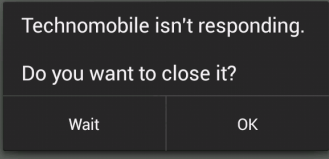
\includegraphics[width=150pt]{img/anr.png}
\begin{itemize}
  \item L'interface graphique ne répond plus
  \item Si le blocage dure plus de x secondes, android affiche ce popup
  \item Il s'agit d'une ANR (application non responding)
  \item Equivalent du ``ne répond pas'' sous windows
\end{itemize}
\end{frame}

\begin{frame}[fragile] 
\frametitle{Le multithreading, notion de thread}
\begin{itemize}
  \item Thread = fil
  \item Fil d'exécution du code
  \item Un thread n'exécute qu'une instruction à la fois
  \item Si du code est long, il bloque le thread
  \item Java s'occupe de répartir les threads sur les coeurs du CPU
\end{itemize}
\end{frame}

\begin{frame}[fragile] 
\frametitle{Le multithreading, le thread UI}
\begin{itemize}
  \item Toutes les instructions de l'IHM s'exécutent dans le même thread
  \item \textbf{Le thread UI (main thread) doit être préservé de tout calcul
  long}
  \item \textbf{Inversement, tout le code touchant à l'UI doit être exécuté dans le thread UI}
  \item Pour les API $>$ 9, possibilité d'activer StrictMode via la classe StrictMode
  \item Sur android 4.0+, possibilité d'activer StrictMode dans les options développeur
\end{itemize}
\end{frame}
\begin{frame}[fragile] 
\frametitle{Le multithreading, créer des threads}
Etape 1 : créer un runnable avec le code à exécuter
\begin{lstlisting}
Runnable code = new Runnable() {
    public void run() {
        //code ici
    }
};
\end{lstlisting}
Etape 2 : lancer un thread exécutant ce runnable
\begin{lstlisting}
new Thread(code).start();
\end{lstlisting}
/!$\backslash$ Ne pas confondre start et run /!$\backslash$
\end{frame}
\begin{frame}[fragile] 
\frametitle{Le multithreading, astuces sous android}
Astuce 1 : Les AsyncTasks
\begin{itemize}
  \item Gère le cycle de vie d'une tâche et exécute chaque méthode dans le bon thread
  \item onPreExecute : thread UI
  \item doInBackground : thread dédié
  \item onPostExecute : thread UI
\end{itemize}
\end{frame}
\begin{frame}[fragile] 
\frametitle{Le multithreading, astuces sous android}
Astuce 2 : Exécuter du code dans le thread UI depuis un autre thread
\begin{itemize}
  \item Pour communiquer entre threads on utilise la classe Handler et on envoie
  des ``messages''
  \item Méthode pratique : runOnUIThread(Runnable) de Activity
  \item Méthode pratique : post(Runnable) de View
\end{itemize}
\end{frame}
\begin{frame}[fragile] 
\frametitle{Validation des groupes / idées de projet}
Pensez à envoyer les idées de projet et les compositions de groupe avant le 28
avril\\
Email : ungawa14@gmail.com
\end{frame}
\end{document}



